\problem{}
The figure shows a flow network in which an $s$-$t$ flow has been computed. The capacity of each edge appears as a label next to the edge, and the numbers in boxes give the amount of flow sent on each edge (edges without boxed numbers have no flow being sent on them).
Find a minimum $s$-$t$ cut in the flow network, and say what its capacity is.
\begin{figure}[htbp]
    \centering
    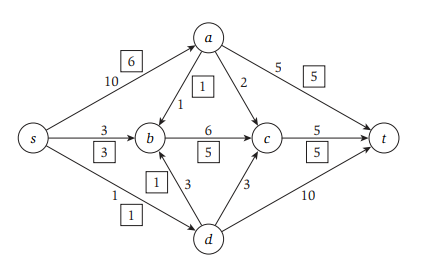
\includegraphics[width=0.8\textwidth]{6.png}
    \end{figure} 

\solution{

}

\newpage
